\chapter{Experiments and results}
Theory shows that internal agent state transparency and the anti-entropy mechanism reward honesty
and punish any strategic manipulation. We implemented this mechanism and establish in this chapter
how it handles strategic manipulation. More specifically we emulate honest agents and multiple 
types of strategic manipulators in small scale experiments. We can observe the behavior of the 
honest agents and find that strategic manipulators are detected and isolated. We show that honest agents who
execute our mechanism are able to effectively detect malicious agents that do not share or do not verify their partners 
and ignore them for future interactions.

The rest of the chapter is structured as follows: we first give an overview of the software 
architecture. Then we explain the setup of the experiments and the types of strategic manipulation
that will be emulated. Finally we present the results of the experiments.

% In the previous chapters we have explored the problem of dissemination of information in distributed
% trust systems. We offered a solution in the form of our multichain based TrustChain architecture, extended 
% it with internal agent state transparency and designed a mechanism that prevents any free-riding on
% dissemination and validation of information on transactions. In this chapter we aim to prove the 
% properties of the mechanism and architecture by experimental analysis. We built a proof-of-concept
% software that fully implements the architecture and mechanism described in this work. It allows us 
% to run an emulation of an agent network and study the behavior of agents in the presence of strategic
% manipulators.

\section{Experiment design}
The goal of the experiments is to prove the true effectiveness of the mechanism at detecting 
manipulation attempts and isolating malicious agents. Three different types of dishonest behavior 
will be analyzed in the experiments.

\begin{itemize}
    \item \textbf{Dissemination free-rider}: An agent that gains an advantage by not 
    expending resources on disseminating transaction records.
    \item \textbf{Verification free-rider}: An agent that gains an advantage by not expending 
    resources on verifying the behavior of their peers
    \item \textbf{Malicious}: An agent that manipulates or withholds information in order to gain an
    advantage. 
\end{itemize}

% The goal of the experimental analysis is to show that free-riding on dissemination and validation of
% transaction information is no longer possible with the extension of TrustChain proposed in 
% chapter~\ref{chap:state_transparency} and the mechanism in chapter~\ref{chap:mechanism}. This would
% be a major step towards a secure and valid distributed trust system. 

In the experiments we emulate small agent networks up to 6 agents. We assume that agents are trying to perform 
interactions with each other. The experiments are not concerned with the actual trust agents have 
in each other so we keep transaction blocks empty. Agents are acting completely autonomously 
but knows about all the other agents in the network. At a frequency of 20 per second agents go through
rounds, in each round an agent has a 1\% chance of starting an interaction. This adds up to approximately
1 transaction every 5 seconds. In addition agents respond to interaction requests from their peers 
asynchronously. At the start of the interaction a peer is selected with uniform probability. If an
interaction with the selected partner is already ongoing, the new interaction request is cancelled
without selecting a new partner. The same happens when the selected partner is a known malicious 
agent. Once the interaction is started honest agents perform according the mechanism as described in
chapter \ref{chap:mechanism}. The other types of agents each have some deviation from the expected
behavior in order to obtain an unfair advantage. All types of agents which were used in the experiments
are listed in Table \ref{tab:agent_types}.

\begin{table}
    \caption{Agent types used in the experiments}
    \label{tab:agent_types}
    \begin{tabular}{p{3cm}|p{3cm}|p{8cm}}
    \textbf{Type} & \textbf{Sub-type} & \textbf{Behavior} \\ \hline \hline
    \multirow{3}{3cm}{ Dissemination free-rider (DFR) } & No exchanges & Does not create any exchanges \\ \cline{2-3}
    & Empty exchanges & Creates exchanges blocks with empty exchanges \\ \cline{2-3}
    & Self-requests & Exchanges only own chain \\ \hline
    Verification free-rider & - & Acts honestly but blindly trusts all partners without verifying their data or behavior \\ \hline
    \multirow{2}{3cm}{ Manipulator } & Hiding transaction & Creates a normal transaction and tries to hide it afterwards \\ \cline{2-3}
    & Forking & Creates two conflicting transactions and shares them with two different peers \\ \hline
    \end{tabular}
\end{table}
    

With these types of agent we run experiments with different sets of agents. In experiments with only
a single dishonest agent, the experiment is successful if the honest agents stay among themselves
and ignore the dishonest agent. That is, the dishonest agent should have 0 transactions at the end
of the experiment. In the case with multiple dishonest agents we have to make a distinction between
multiple single acting dishonest agents and collaborating groups of dishonest agents. 

\section{Implementation details}

The experiments are run on a standalone implementation of TrustChain with the mentioned extension
and mechanism. The code is available through GitHub\footnote{https://github.com/jangerritharms/aupair}.
The code is based on the TrustChain implementation of py-ipv8\footnote{https://github.com/tribler/py-ipv8}
another project that is developed in the context of BlockchainLab. 

The implementation is done in Python. The programming language was chosen as it allows for fast development,
offers many useful extensions and the py-ipv8 dependency is also written in Python. At the core of
the software is the \texttt{agent} module. It implements the agent base class which contains all 
functionality for communicating with other agents. They communicate with each other using tcp sockets, 
implemented using the \texttt{zeromq} library. Messages for the communication are defined in the 
Google \texttt{protobuf} format. The basic TrustChain data structures and block database implementation
were taken from the \texttt{py-ipv8} project. Next to the agents there is the discovery 
server which handles the peer discovery process. 

The experiment is started by spawning all agent processes and the discovery server. Once the agent 
process is started each agent sends a registering message to the discovery server to register the 
public key with the address of the tcp endpoint. After a 5 second initialization period it is assumed
that all processes have started and registered. The discovery server then sends a message to all 
registered agents containing their peers. Once that messages is received agents start running the
experiment. 

\section{Experiment results}
In the following we will present the results of our experimental analysis.
\subsection{Dissemination free-riders}

\begin{figure}
    \centering
    \begin{subfigure}{\textwidth}
      \centering
      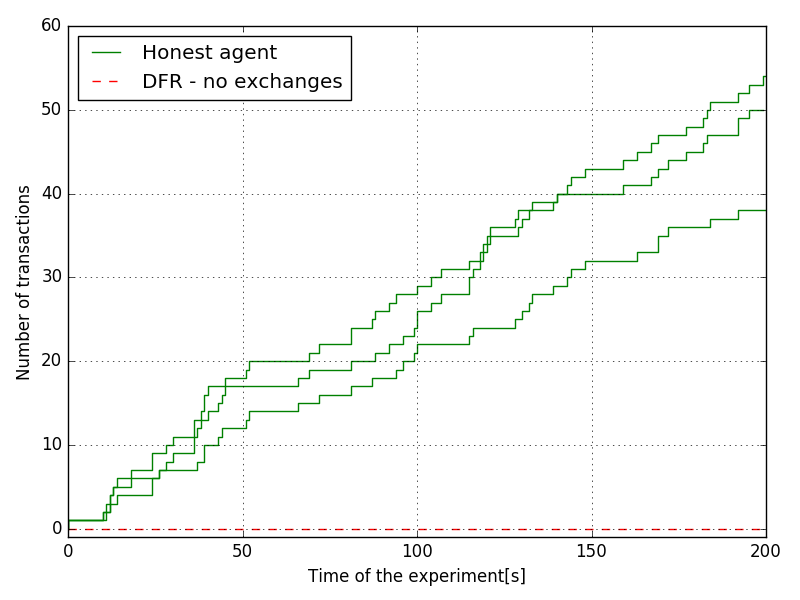
\includegraphics[width=.6\linewidth]{images/DFR_no_exchanges}
      \caption{Transactions over time of honest agents with dissemination free-rider that does not 
      perform any exchanges}
      \label{fig:DFR_no_exchanges}
    \end{subfigure}\\
    \begin{subfigure}{\textwidth}
      \centering
      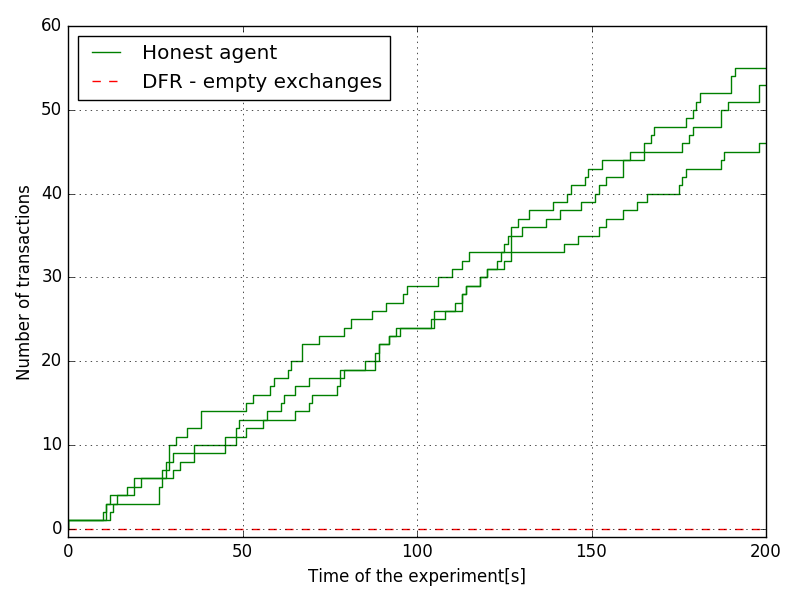
\includegraphics[width=.6\linewidth]{images/DFR_empty_exchanges}
      \caption{Transactions over time of honest agents with dissemination free-rider that creates 
      empty exchanges}
      \label{fig:DFR_empty_exchanges}
    \end{subfigure}\\
    \begin{subfigure}{\textwidth}
        \centering
        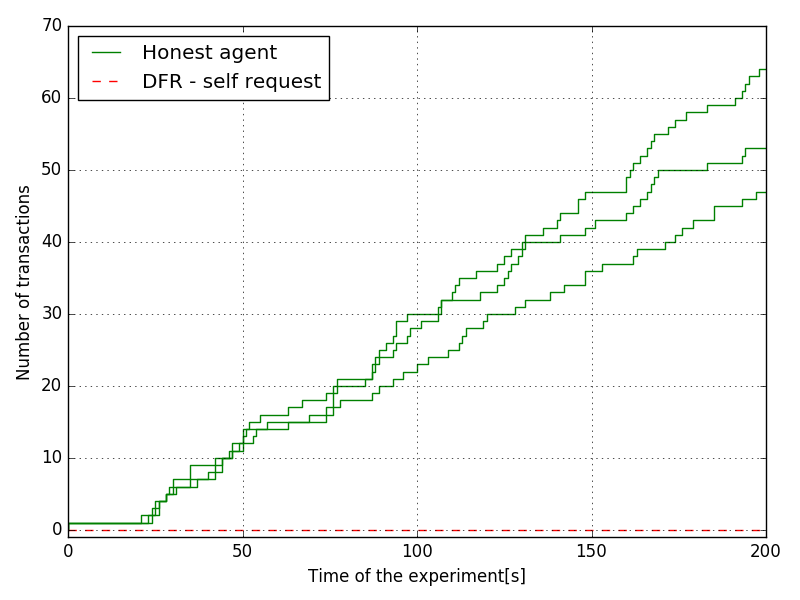
\includegraphics[width=.6\linewidth]{images/DFR_self_request}
        \caption{Transactions over time of honest agents with dissemination free-rider that only 
        exchanges own data}
        \label{fig:DFR_self_request}
      \end{subfigure}
    \caption{Transactions over time of three experiments with different types of dissemination 
    free-riders}
    \label{fig:DFR}
\end{figure}

The first experiment to run is concerning the dissemination free-riders. One desired property of the 
internal agent state transparency is that disseminating information is strategy-proof. That means, 
it should not be advantageous to not share information. In this first set of experiments we observe
the behavior of three honest agents in the presence of three different types of dissemination 
free-riders. Figure \ref{fig:DFR} shows the number of transactions of each agent against the time of
the experiment.

All experiments show the same general picture: all honest agents steadily increase their succesful 
interactions throughout the experiment and end up between 40 to 60 transactions. The dishonest agents 
are not able to perform a single interaction. As expected 
the dissemination free-riders have no chance to interact with the honest agents in any 
of the three cases. That means the honest agents detect the wrong behavior of their malicious peers
and ignore them for future interactions.

In the first experiment \ref{fig:DFR_no_exchanges} the 
dishonest agent does not exchange any data and therefore does not create any proof of exchanges. Yet
in order to interact with honest agents the dissemination free-rider needs to publish a complete 
chain. Honest nodes detect the lack of exchange blocks upon inspection and subsequently distrust 
that agent.

The second experiment \ref{fig:DFR_empty_exchanges} the dishonest agent aims to create empty exchanges.
In the role of the responder, the agent requests no blocks from the honest agents and as initiator 
the agent tries to claim that no blocks were received from the honest agent. However, as explained
in the theory section, empty exchanges are not possible because agents always have at least one new
block to talk about. Also agents only sign an exchange block if they agree with the hash of transferred
blocks. That is, if the dishonest agent claims no blocks were sent but actually the honest agent did
send data, the honest agent will not sign the block. That way, also in this case the honest agents
are able to detect the wrong behavior.

Finally, the third type of dissemination free-riders, results shown in Figure\ref{fig:DFR_self_request}
, requests and sends data about itself but not any other knowledge. When in the responder position, 
the agent can request only its own blocks. As initiator the agent tries to act again as if no data
was received other than its own blocks. However the partner can see that the exchange block proposal
does not properly represent the data exchanged and will therefore stop the transaction. Also this way
the agent is not able to interact with honest partners. 

We find that dissemination free-riding leads to isolation and no transaction with honest partners. 
That means no reputation or trust will be build with this type of misbehaving agents and any hope for
future rewards is voided. Agents have to disseminate their data in order to be accepted and to prosper.

\subsection{Collaborating dissemination free-riders}
The situation changes when multiple dissemination free-riders join forces and collaborate in creating
a subnetwork. This situation can arise if a software is forked and an alternative release is published
which does not contain any data exchanges. In order to analyze this situation we ran an experiment 
with three honest agents and three dissemination free-riders. The transactions are plotted against 
time in Figure \ref{fig:50percent}.

\begin{figure}[h!]
    \centering
    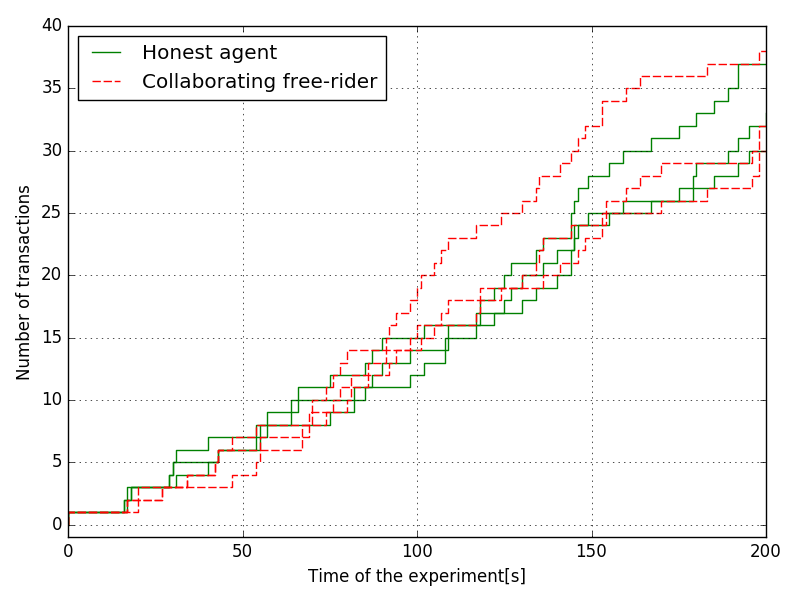
\includegraphics[width=0.7\textwidth]{images/50percent}
    \caption{Transaction history of three honest agents and three dissemination free-riders
    that are cooperating}
    \label{fig:50percent}
\end{figure}

\begin{figure}[h!]
    \centering
    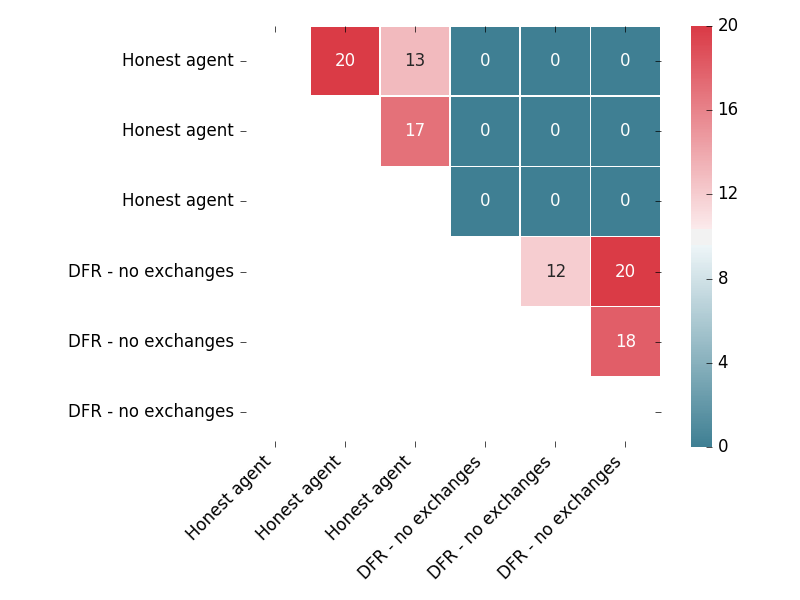
\includegraphics[width=0.7\textwidth]{images/50percent_interaction_matrix}
    \caption{Interaction matrix of three honest agents and three dissemination free-riders who are cooperating}
    \label{fig:50percent}
\end{figure}

\subsection{Malicious behavior}

\begin{figure}
    \begin{subfigure}{\textwidth}
      \centering
      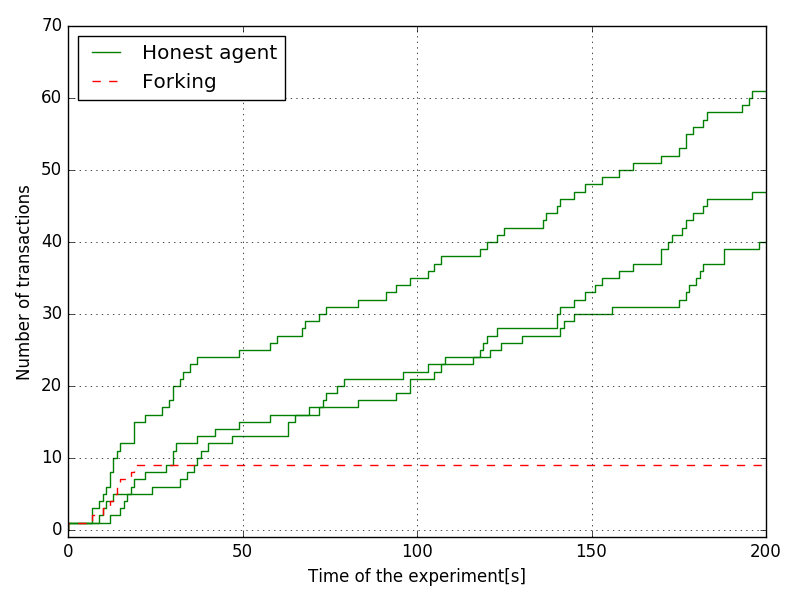
\includegraphics[width=.6\linewidth]{images/forking}
      \caption{Transaction history of three honest agents interacting with one strategic manipulator who performs a fork}
      \label{fig:forking}
    \end{subfigure}\\
    \begin{subfigure}{\textwidth}
      \centering
      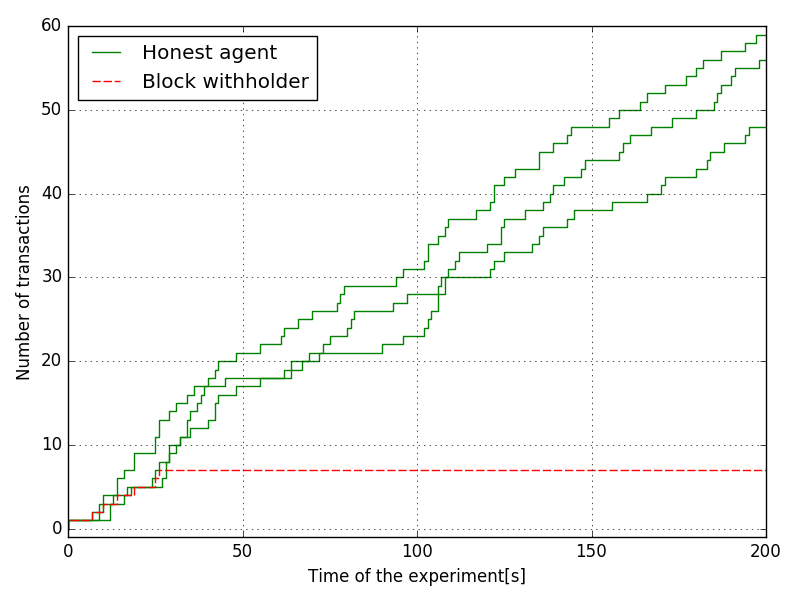
\includegraphics[width=.6\linewidth]{images/transaction_hiding}
      \caption{Transactions over time of three honest agents with one strategic manipulator who tries to hide a transaction}
      \label{fig:DFR_empty_exchanges}
    \end{subfigure}\\
\end{figure}

\subsection{Verification free-rider}

\begin{figure}
    \begin{subfigure}{\textwidth}
      \centering
      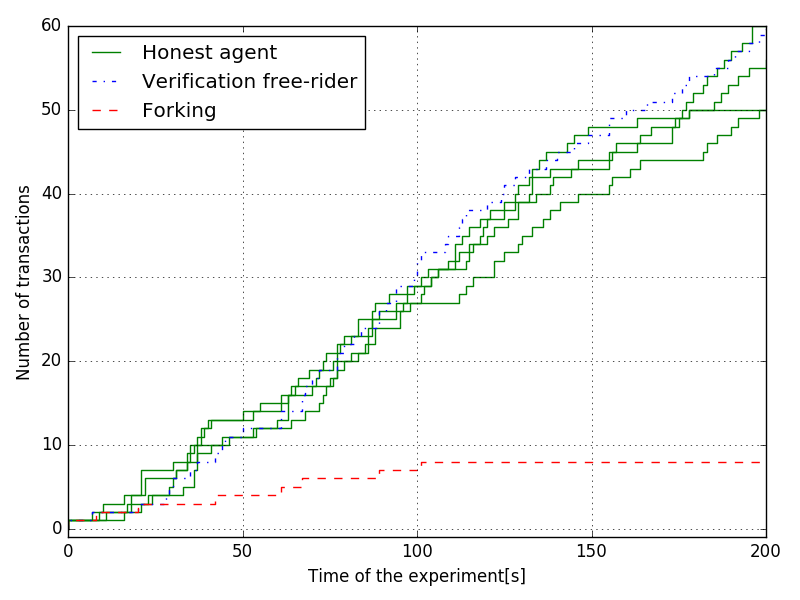
\includegraphics[width=.6\linewidth]{images/verification_doublespend_honest}
      \caption{Transaction history of three honest agents interacting with one strategic manipulator who performs a fork and a verification free-rider}
      \label{fig:verification_doublespend_honest}
    \end{subfigure}\\
    \begin{subfigure}{\textwidth}
      \centering
      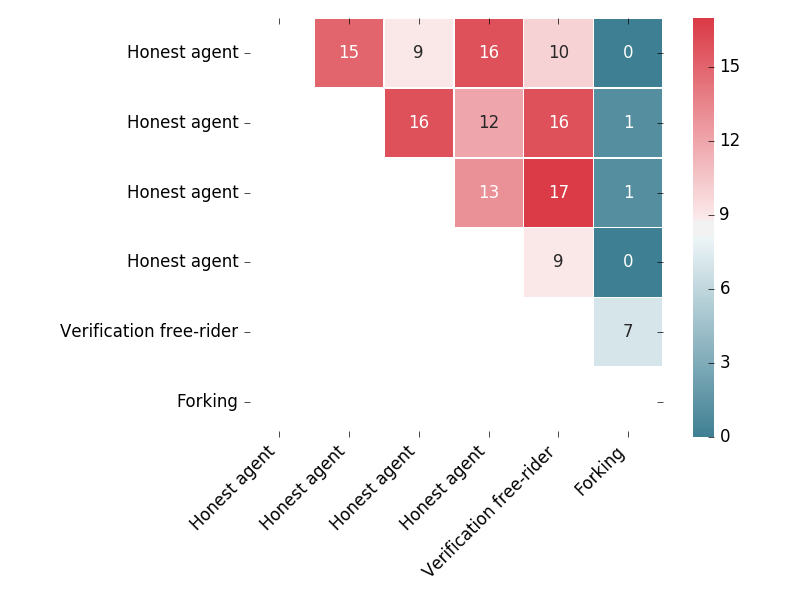
\includegraphics[width=.6\linewidth]{images/verification_doublespend_honest_matrix}
      \caption{Interaction matrix of three honest agents with one strategic manipulator who performs a fork and a verification free-rider}
      \label{fig:verification_doublespend_honest_matrix}
    \end{subfigure}\\
\end{figure}

\begin{figure}
    \begin{subfigure}{\textwidth}
      \centering
      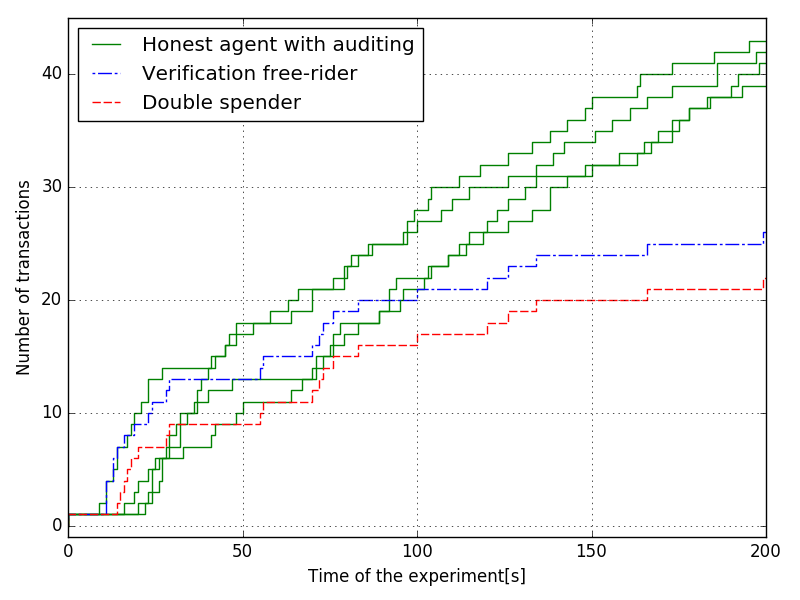
\includegraphics[width=.6\linewidth]{images/verification_doublespending}
      \caption{Transaction history of three honest agents with replay verification interacting with one strategic manipulator who performs a fork and a verification free-rider}
      \label{fig:verification_doublespending}
    \end{subfigure}\\
    \begin{subfigure}{\textwidth}
      \centering
      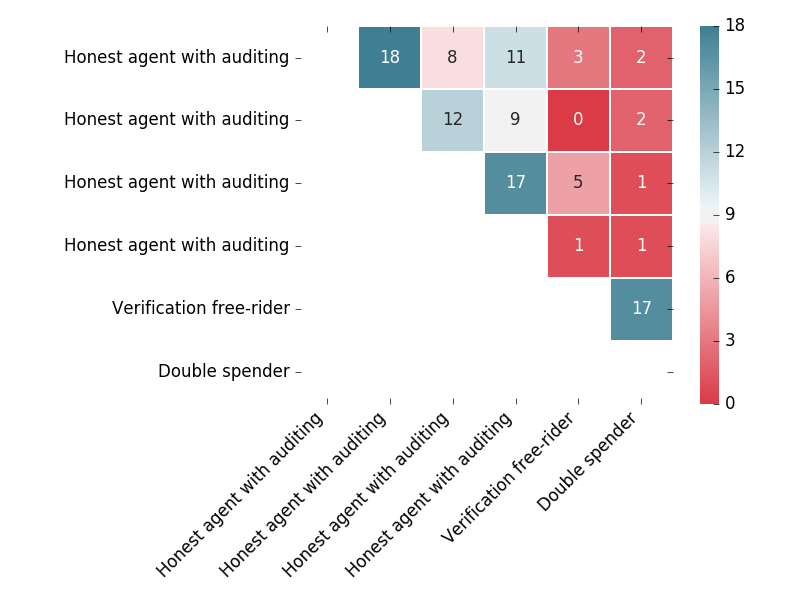
\includegraphics[width=.6\linewidth]{images/verification_doublespending_matrix}
      \caption{Interaction matrix of three honest agents with replay verification with one strategic manipulator who performs a fork and a verification free-rider}
      \label{fig:verification_doublespending_matrix}
    \end{subfigure}\\
\end{figure}

\section{}

\subsection{Sybil attack}